\section{Databehandling}
\subsection{Afbildning med én samlelinse}
I dette forsøg, ændres positionen for linsen hvorefter positionen af skærmens position ændres, så billedet igen står skarpt. Der ønskes altså at undersøge sammenhængen mellem \cref{eq:formel}.
Vores resultater kan ses på
\begin{table}[H]
    \begin{tabular}{c|c|c|c|c|c|c|c|c|c|c}
        58 &  64 &  59 &  57 &  57 &  57  & 59  & 61  & 62  & 63  & 66
    \end{tabular}
    \caption{}
    \label{}
\end{table}
\begin{figure}[H]
    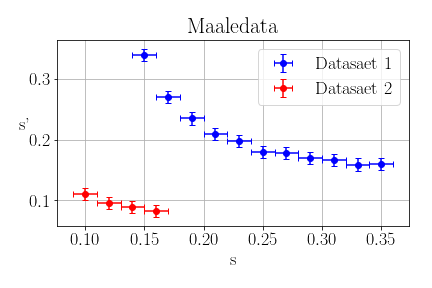
\includegraphics[width=\linewidth]{usikkerhed.png}
    \caption{}
    \label{fig:usikkerhed}
\end{figure}

\begin{figure}[H]
    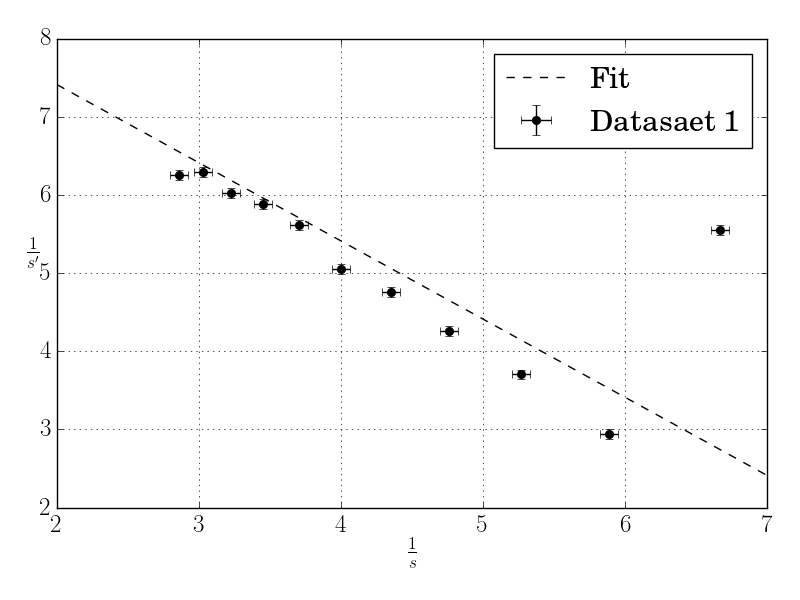
\includegraphics[width=\linewidth]{1.png}
    \caption{}
    \label{fig:1}
\end{figure}

\begin{figure}[H]
    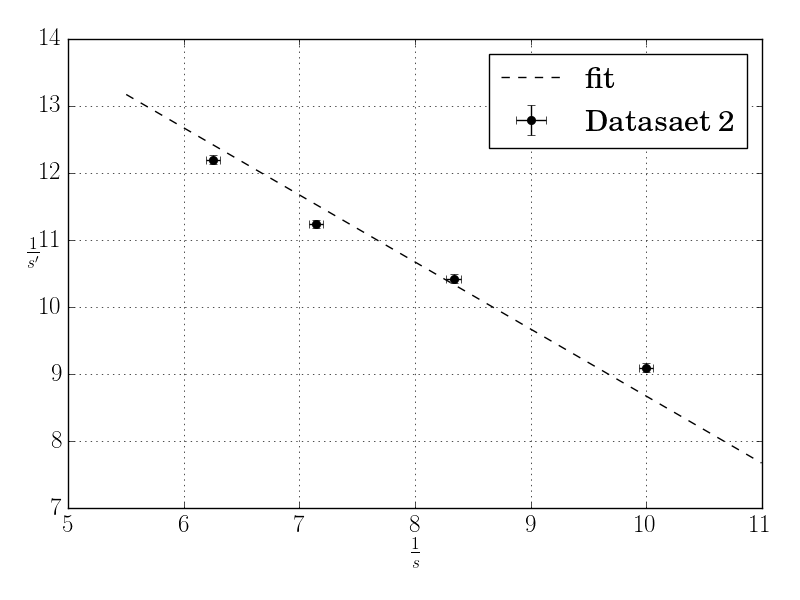
\includegraphics[width=\linewidth]{2.png}
    \caption{}
    \label{fig:2}
\end{figure}

\begin{figure}[H]
    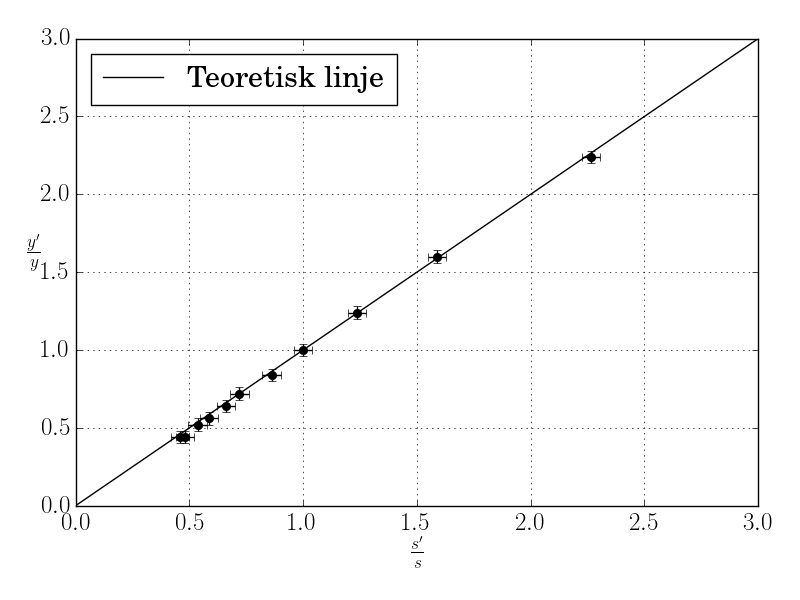
\includegraphics[width=\linewidth]{3.png}
    \caption{}
    \label{fig:3}
\end{figure}
